
\chapter{Contextualización}\label{chapter:context}

En este capítulo se revisan los temas y conceptos relevantes para el desarrollo del trabajo. Se formaliza la definición de robot doméstico y sus alcances. Se describe la memoria humana, sus categorías, funcionamiento y procesos cerebrales relevantes. Basando en los temas anteriores, se revisa la relación entre robótica y la memoria humana: se describen los distintos enfoques existentes, las reglas generales para su implementación y los frameworks actuales. Finalmente, se detalla el software de interés y las plataformas objetivo del proyecto.

% ================================================================
% ================================================================
% ================================================================

\section{Robots de servicio}

La Federación Internacional de Robótica (IFR)\cite{IFR} define \textit{robot} como:
\begin{quotation}
``Un mecanismo actuado y programable en dos o más ejes y con un cierto grado de autonomía, que se mueve en su entorno para realizar tareas previstas. En este contexto, autonomía se refiere a la habilidad de realizar tareas previstas, basado en el estado actual y lo sensado, sin intervención humana.''
\end{quotation}

Asimismo, la IFR define un \textit{robot de servicio} como un robot ``que realiza tareas útiles para humanos o equipamiento, excluyendo aplicaciones de automatización industrial''. Así, un robot de servicio debe trabajar en ambientes no controlados y con la autonomía suficiente que le permita llevar a cabo su cometido. Generalmente, la robótica de servicio se enfoca en asistir a los seres humanos en tareas repetitivas y comunes.

Según su área de aplicación, un robot de servicio se clasifica en \textit{de uso personal} o \textit{de uso profesional}. Los primeros son utilizados en ambientes no comerciales y por personas comunes; como por ejemplo, un robot sirviente o una silla de ruedas autónoma. Un robot de servicio profesional se utiliza en ambientes comerciales, usualmente operados por alguien entrenado; un ejemplo son los robots de entrega de paquetes o para cirugía.


\subsection{Robots Domésticos}\label{sec:domestic_robots}

Según la recopilación de datos realizada por la IFR durante el 2016, este tipo de robots es utilizado en las siguientes áreas:
\begin{itemize}[topsep=0pt]
\setlength\itemsep{0.2em}
\item Tareas domésticas: De compañía, asistencia, limpieza, cuidado del hogar.
\item Entretenimiento: Juguetes, comunicación, educación e investigación.
\item Asistencia a ancianos y discapacitados: Sillas robóticas y robots para cuidar personas.
\item Transporte.
\item Seguridad y vigilancia.
\item Otros que no caen en las categorías anteriores.
\end{itemize}
\bigskip

El foco de este trabajo son los robots de servicio personales, dedicados a tareas domésticas, clasificación a la que en  adelante se referirá como \textit{Robots Domésticos}.

Para entender el alcance del trabajo, en cuanto a qué es lo que se espera del sistema, a continuación se listan algunas capacidades de los robots domésticos. Un robot de compañía y asistencia tiene, pero no se limita a las siguientes tareas:
\begin{itemize}[topsep=0pt]
\setlength\itemsep{0.2em}
\item Interacción amistosa con humanos.
\item Ayudar a recordar y organizar tareas.
\item Cooperar con la realización de un procedimiento.
\item Guiar y seguir a personas.
\item Recordar información y entidades.
\end{itemize}
\bigskip

Algunas tareas que robots domésticos de tipo mayordomo deben ejecutar son:
\begin{itemize}[topsep=0pt]
\setlength\itemsep{0.2em}
\item Ofrecer comida y bebestibles.
\item Preparación de comida.
\item Ordenar y limpiar el hogar.
\end{itemize}
\bigskip


% ================================================================
% ================================================================
% ================================================================

\section{Memoria Humana}

\todo[inline]{Poner referencias a todo esto. ... psicoanalisis ... ciencias cognitivas.}
% \cite{Deutsch2008} 

La memoria es un elemento fundamental para los humanos en su día a día, es parte integral de su existencia. Permite recordar quién, qué, cómo, dónde y cuándo. En términos psicológicos, es la habilidad para para codificar, almacenar y luego obtener información sobre eventos pasados, en el cerebro. Los pensamientos son parte de la memoria de corto plazo, mientras que eventos pasados son almacenados en una memoria de largo plazo. Existen muchos estudios en el área de la psicología cognitiva con diversas descripciones y modelos teóricos de cada tipo de memoria\cite{Vijayakumar2014}.

Desde el punto de vista de la información procesada, la memoria es vista como una facultad humana consistente en procesos para el manejo de información. Los 3 componentes principales son:

\begin{itemize}[topsep=0pt]
\setlength\itemsep{0.2em}
\item Codificación: En este paso, se adquiere nueva información desde los sentidos humanos. Los datos son convertidos a un formato que pueda ser almacenado en la estructura cerebral correspondiente.
\item Almacenamiento: Consiste en la creación de registros permanentes de información. Es un proceso pasivo, de continuo procesamiento para clasificar datos nuevos y los ya existentes en el cerebro.
\item Adquisición: Hace referencia al acceso de datos almacenados. El proceso se realiza en el momento, para obtener una reconstrucción aproximada de la información, a partir de elementos repartidos en distintas partes del cerebro.
\end{itemize}
%\bigskip


La memoria puede ser dividida en múltiples sistemas de independientes, con funcionalidades bien definidas y sustentados por distintas estructuras cerebrales. La primera diferenciación define dos tipos de memoria: la memoria de corto y la de largo plazo, STM (Short-Term Memory) y LTM (Long-Term Memory), por sus siglas en inglés. En el diagrama de la figura \ref{img:human_memory} se muestra una separación clásica utilizada en el área de las ciencias cognitivas\cite{Eichenbaum:2008}, explicada en las siguientes subsecciones.

\begin{figure}[H]
\centering
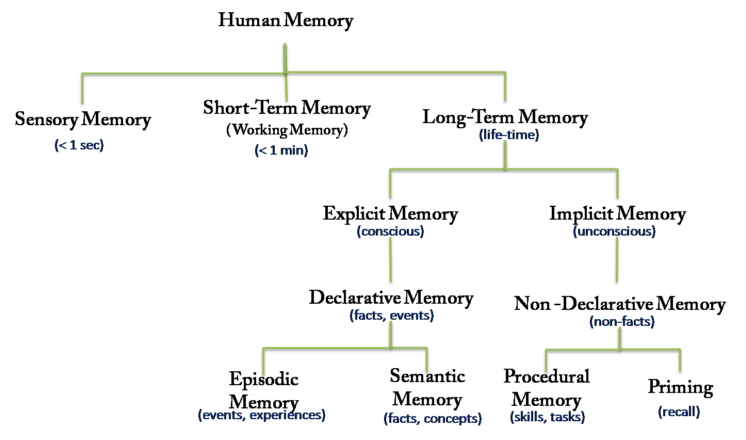
\includegraphics[width=0.8\textwidth]{./figures/diagrama_memoria.png}
\caption{\small Clasificaciones de la memoria humana. Obtenido de \cite{Vijayakumar2014}.}
\label{img:human_memory}
\end{figure}

% Sobre el estudio de la memoria.. origenes.. Tulving 

\subsection{Memoria de Corto Plazo}

En el ámbito cognitivo, la STM se refiere a la habilidad de estar atento, recopilar información  y memorias, para luego utilizarlas dentro de un corto periodo de tiempo. Es responsable de almacenar información constantemente y de decidir que parte será transferida a la memoria de largo plazo. El término de \textit{Memoria de Trabajo} suele ser utilizado de manera intercambiable con el de STM. Además, suele ser agrupada con otro tipo de memoria, llamada \textit{Sensorial}.

La STM se caracteriza por manejar información muy detallada, ser de poca capacidad y permitir un rápido acceso a estos datos. Permite recordar rápidamente y con gran detalle experiencias ocurridas hace pocos segundos, pero con dificultad creciente a medida que avanza el tiempo.

Se sustenta principalmente en la corteza prefrontal del cerebro. Algunos estudios han mostrado que las neuronas involucradas son capaces de mantener información relevante de corto plazo, la que es combinada con información sensorial entrante y áreas que manejan la toma de decisiones. %(Miller, 2000).
En los humanos esta área presenta gran activación durante procesos de codificación, acceso y manipulación de memorias. %(Postle, 2006). 


\subsection{Memoria de Largo Plazo}

La LTM se asocia al almacenamiento permanente de información en el cerebro. Se caracteriza por manejar mucha información sobre experiencias y entidades, ser menos detallada y proveer un acceso más lento a los recuerdos, respecto a la STM\cite{Eichenbaum:2008}. Cierta información de la STM eventualmente es transferida a la LTM. De acuerdo a la figura \ref{img:human_memory}, sus dos principales categorías son la \textit{Memoria Implícita} y la \textit{Memoria Explícita}.
% algunos creen que no está limitada en su capacidad de almacenar información.

\subsubsection{Memoria Implícita}

La memoria implícita  abarca la capacidad de aprender habilidades, hábitos y preferencias, caracterizados por ser mejorados o adquiridos sin una recolección consciente. Así, también suele ser denominada \textit{memoria inconsciente} o \textit{memoria no declarativa}, pues comprende acciones que pueden ser realizadas sin pensar en ellas. Ejemplos de esto, son el andar en bicicleta o tocar un instrumento musical.

Se puede clasificar en \textit{memoria procedural} (P-LTM) y en \textit{memoria de primado}. La primera ayuda a realizar tareas sin pensar en ellas, es decir, maneja el conocimiento del \textit{Cómo}; Ejemplos de esto son comer y caminar. La memoria de primado hace referencia a la predisposición para recordar hechos o información a la que un sujeto es expuesto con anterioridad; Ejemplos de esto son la facilidad para recordar canciones escuchadas hace poco tiempo, o el uso de palabras e ideas vistas recientemente.

Se ha mostrado que la P-LTM se sustenta en el cerebelo, mediante la activación de este durante el uso de habilidades motoras.

Otro tipo de memoria implícita es la \textit{memoria emocional} (Em-LTM). Se encarga de dar significado afectivo a ciertos  estímulos, que de otra forma serían neutrales. Las estructuras cerebrales involucradas son la amígdala, áreas corticales y subcorticales. Esta memoria se expresa mediante la activación del hipotálamo, en conjunto al sistema nervioso simpático, generando reacciones emocionales y sentimientos.


\subsubsection{Memoria Explícita}

La memoria explícita suele ser denominada \textit{memoria consciente} o \textit{memoria declarativa}, pues maneja conocimientos relacionados a hechos y eventos adquiridos de forma consciente. Según las estructuras cerebrales involucradas, se conforma de la \textit{memoria episódica} y de la \textit{memoria semántica}.

La memoria episódica (Ep-LTM) es de carácter  autobiográfico y almacena detalles de eventos y experiencias pasadas. Permite responder a las preguntas ``Qué sucedió'', ``Dónde ocurrió'' y ``Cuándo ocurrió''. Un humano puede acceder a esta memoria si es capaz de decir: ``recuerdo que''. Este tipo de memoria da al ser humano la sensación de continuidad en el tiempo.

La memoria semántica (S-LTM) almacena el conocimiento de hechos, significados, categorías y proposiciones. Un humano puede acceder a esta memoria si es capaz de decir: ``sé que''. Esta memoria se abstrae de perspectiva e información situacional.

Las estructuras cerebrales que soportan la memoria explícita son el hipocampo, encargado de manejar la Ep-LTM, junto a la corteza cerebral, en donde se distribuyen los conocimientos de la S-LTM. En el hipocampo se mantienen conexiones neuronales a los sectores de interés de la corteza, en donde se alojan conocimientos semánticos asociados a cada episodio.

Un ejemplo de uso de Ep-LTM es el recuerdo de una graduación escolar, el lugar y la fecha donde ocurrió. La S-LTM podría responder en que consiste una graduación y describir la ropa que se suele ocupar en ellas.


\subsection{Plasticidad Sináptica y Modulación}

Se denomina \textit{consolidación} de memoria al proceso de transición de conocimiento desde la STM a la LTM. Durante la consolidación se generan conexiones neuronales entre la Ep-LTM y la respectiva zona semántica. Para activar la consolidación se requiere de un estímulo relevante, sumado a la cadena de eventos para el almacenamiento.

Se denomina \textit{deterioro} de memoria u ``olvido'' al proceso de debilitamiento de las conexiones neuronales establecidas por los procesos de consolidación. Está en constante funcionamiento, degenerando las asociaciones entre la Ep-LTM y la S-LTM. Por lo tanto, en este contexto, el olvido no significa una eliminación de los datos en el cerebro, sino que estos siguen ahí, pero la conexión requerida es inexistente o es demasiado débil para poder ocuparla.

Existen procesos químicos a nivel cerebral que afectan la consolidación y el deterioro de la LTM. Hay evidencia de que estos están en continuo funcionamiento. Estos eventos celulares ocurren en una escala de segundos a minutos, y son esenciales para la mantención de la memoria a largo plazo.

Es posible modular ambos procesos. Las experiencias repetidas potencian la consolidación de la memoria, lo que fortalece las conexiones neuronales. Por otro lado, la memoria emocional es capaz de potenciar o deprimir las reacciones químicas requeridas; según los estímulos a los que se enfrente, modifica el nivel de relevancia de los eventos, pudiendo generar memorias muy fuertes y hábitos arraigados. Ejemplos de esto, son la memorización por repetición, los flashbacks y las memorias asociadas a eventos importantes como cumpleaños.

% ================================================================
% ================================================================
% ================================================================

\section{Memoria y robótica}

En esta sección se presenta el estado del arte respecto al uso de LTM en robótica. En primer lugar se presenta la importancia de la LTM y las expectativas para un robot doméstico. Luego se hace una comparación entre la memoria humana y el manejo de información en robots.  Se presenta el estado del arte para cada componente cognitivo de interés. Finalmente, se describen otros enfoques de la literatura para la implementación de LTMs, que no están basados en el enfoque biológico utilizado en este proyecto.


\subsection{Relevancia de la memoria robótica}

La memoria es una habilidad esencial para cualquier ser social. Lo mismo aplica para un robot doméstico cuya misión sea establecer una relación de largo plazo con usuarios humanos. Un problema común es que los usuarios tienden a perder el interés rápidamente en los robots, debido a la falta de vida y expectativas no cumplidas, respecto a la inteligencia y capacidad de socializar de la máquina. El problema se potencia con el paso del tiempo, donde la motivación por interactuar disminuye y se genera frustración, a medida que el robot continua repitiendo los mismos comportamientos predefinidos\cite{Ho2009}.

Si se desea mejorar la interacción humano-robot, entonces se requiere que el robot se comporte de manera más natural. Los mejores agentes robóticos sociales deberían satisfacer las necesidades cognitivas y sociales humanas; mientras más familiar sea la interacción, serán más efectivos en su propósito. Así, la LTM es una habilidad crucial si se espera que el robot sea capaz de aprender y adaptarse a su entorno.


Por otro lado, desde un punto de vista práctico, se ha mostrado que el concepto de memoria LTM aplicada a robots es beneficioso. En \cite{Salgado2012} ocupan memoria P-LTM para mejorar el desempeño de un robot en ambientes dinámicos, logrando acelerar el proceso de adaptación al entorno y la toma de decisiones.

%... blabla util \cite{Vijayakumar2014}


\subsection{Relación entre memoria humana y memoria robótica}


Son muchos los trabajos en LTM que han basado su desarrollo en la taxonomía de la memoria humana, donde se implementan esquemas de información con módulos análogos a los presentados en la figura \ref{img:human_memory}. Esto se puede justificar por la similitud de cada tipo de memoria, con módulos preexistentes en la arquitectura robótica. A continuación se presenta una comparación entre cada tipo de memoria, sus procesos y el análogo robótico.

\subsubsection{Memoria STM}

Se relaciona a todos los datos que están actualmente cargados en la memoria primaria de la máquina. Esta memoria es la utilizada para solucionar la tarea actual, es equivalente a los pensamientos del robot y cumple con las características de la STM humana: es volátil, de rápido acceso y limitada en capacidad. También se encuentra presente en todo archivo temporal manejado por el sistema, mientras está en funcionamiento. Así, la estructura equivalente a la cerebral sería principalmente la RAM de la máquina.


\subsubsection{Memoria S-LTM}

La memoria S-LTM es común y se puede asociar a casi toda fuente de datos estática, no utilizada por las otras memorias. Luego, la S-LTM se sustenta en la memoria secundaria, cumpliendo las características de la LTM humana: es persistente, de acceso costoso y virtualmente ilimitada en capacidad. Algunos ejemplos son:
\begin{itemize}[topsep=0pt]
\setlength\itemsep{0.2em}
\item Bases de datos.
\item Directorios con imágenes de personas y objetos conocidos.
\item Mapa con descripción del ambiente.
\item Frases predefinidas que puede decir el robot.
\item Archivos de audio utilizados por el robot.
\item En general, todo archivo con datos persistentes, cargados en cada sesión de trabajo.
\end{itemize}


\subsubsection{Memoria P-LTM}

Este tipo de memoria es comparable a algoritmos predefinidos para realizar acciones, generalmente motoras. 

Algunos ejemplos comparables son: 
\begin{itemize}[topsep=0pt]
\setlength\itemsep{0.2em}
\item Algoritmos basados en redes neuronales, entrenados para manipular objetos o reconocer patrones.
\item Algoritmos entrenados para tareas específicas, cómo la detección de caras o el reconocimiento de voz.
\item Controladores basados en puntos de operación para acciones motoras.
\item Síntesis de voz
\end{itemize}

Las estructuras equivalentes a la versión cerebral serían los archivos con parámetros para cada algoritmo, obtenidos a partir del entrenamiento o ajustados manualmente.


\subsubsection{Otros tipos de memoria}

Generalmente, tanto STM, S-LTM como P-LTM son un requisito mínimo para el funcionamiento de un software robótico, por lo que no son implementadas conscientemente. Luego, la existencia de tales memorias, no implica la intención de crear una arquitectura LTM similar a la humana. Los otros tipos de memorias sólo son implementados en casos especializados.



\subsection{Memoria LTM explícita}\label{sec:ltm_exp}

\todo[inline]{Sobre approaches para crear memorias episódicas.}
%Han existido diversos intentos por crear memorias episódicas y semánticas. ... tal persona hizo tal cosa .... desde el 2000


\todo[inline]{Sobre los diseños de consolidación utilizados en la literatura.. son pocos :(}

No existe un consenso sobre los contenidos, el formato o las herramientas para implementar Ep-LTM.
%... que recordar y cuando \cite{Kasap2010}
%... modelo de contexto \cite{Sanchez:2015} FELIX
% ... Considerar unificación de información.. que pasa si almaceno obj1 y obj2, pero luego aprendo que son el mismo?
%...... S Memory.. se abstrae de perspecttiva y cosas situacionales \cite{Stachowicz2012}
Sin embargo, si existe una aceptación generalizada sobre los requerimientos mínimos y deseables para el diseño\cite{Vijayakumar2014, Ho2009,  Stachowicz2012, Jockel2008}:

%\subsubsection{Aspectos de diseño}

\paragraph{Aspectos de diseño requeridos:}

% Stachowicz2012
% The first three requirements are given by the criteria of Clayton et al [14]

% corregirlos

\begin{enumerate}[topsep=0pt]
\setlength\itemsep{0.2em}
\item Contenido: (R1) Información de eventos pasados debe ser recolectada e indexada respecto a su contexto espacio-temporal: Qué, dónde y cuándo pasó.

\item Estructura: (R2) Cada evento en conjunto con su contexto espacio-temporal forman una única representación integrada, que debe ser recordada como un todo, en caso de obtener cualquiera de las características del evento.

\item Flexibilidad: (R3) La información almacenada es declarativa por naturaleza, y puede ser flexiblemente almacenada. Particularmente, puede interactuar con conocimiento semántico, incluso si este fue obtenido con posterioridad a la codificación del episodio.

\item Datos específicos: (R4) Memoria episódica cuenta con sólo una instancia de cada evento para su entrenamiento, pues cada evento tiene características específicas a la situación.

\item Ep-LTM es LTM y declarativa: (R5) La memoria episódica es una forma de memoria LTM. Puede almacenar recuerdos por segundos, minutos, días o años. También es una forma de memoria declarativa.

\item Perspectiva: (R6) Memoria episódica debe lidiar con datos específicos al evento, lo que implica una perspectiva. Es decir, eventos recordados deben mantener la misma perspectiva que se tenía en la experiencia original.

\item Anidamiento: (R7) Eventos almacenados en la memoria episódica pueden variar en tiempo y extensión. Particularmente, pueden ocurrir eventos dentro del actual.

\item Trasposición : (R8)  Eventos almacenados en la memoria episódica pueden variar en tiempo y extensión. Particularmente, un evento A puede iniciar antes B, pero terminar durante la vida de B.

\end{enumerate}

\paragraph{Aspectos de diseño deseables:}

\begin{enumerate}[topsep=0pt]
\setlength\itemsep{0.2em}
\item No intrusivo: (R9) El campo ``Qué'' puede contener información aleatoria, que se puede proveer mediante diversos módulos de software. Se espera que la LTM no requiera dependencias de módulos externos para poder funcionar y representar los datos. A la vez, no puede depender en que los otros módulos no cambien la representación de sus datos.

\item Eficiente: (R10) El sistema debe ser lo suficientemente eficiente para tolerar el manejo de una alta tasa de eventos, sin degradar el funcionamiento del robot.

\item Escalable: (R11) Los costos de manejo de la información deben escalar bien, independientemente de la cantidad de tiempo de operación.
\end{enumerate}



\subsubsection{Procesos de consolidación y deterioro}
%
%- algunos solo procuran desarrollar reglas sobre como actualizar los pesos de aprendizaje
%- dejar de aprender (sorprenderse al ser mayor)
%... modelo probabilistico para consolidar y decaer \cite{Dodd2005}
%... olvidar cosas.. si no se implementa, entonces la busqueda de informacion seria cada vez mas compleja. \cite{Deutsch2008}
%... reglas de consolidacion \cite{Dodd2005}

En un esquema LTM, un episodio puede estar constituido de muchos eventos, pero no todos son igualmente relevantes. En su trabajo, Kelley \cite{Kelley2014} estudia 3 estrategias para la consolidación de recuerdos. La primera almacena todo lo ocurrido, pero tiene un costo de búsqueda lineal, respecto a los episodios almacenados; esta estrategia es impráctica a largo plazo. La segunda sólo almacena eventos interesantes y realiza una búsqueda entre los más recientes; esta estrategia es práctica, pero no permite abstracción del evento. La tercera estrategia se basa en un postprocesamiento de las memorias, de manera similar al sue\~no humano.

La estrategia propuesta por Kelley se basa en recordar todo, pero realizando un postprocesamiento de los datos una vez terminado el evento. La ventaja es que no sólo permite recordar episodios, sino que además permite reconocer pistas o estímulos previos que sirven para prevenir un evento indeseado o potenciar eventos interesantes. Además, permite almacenar eventos posteriores, que sirven para entender las consecuencias del evento de interés. 

En la figura \ref{img:sleep_eventos} se muestra un episodio de interés y sus eventos previos y sucesivos. La memoria almacena la secuencia completa de eventos. En el postprocesamiento se descartan los elementos poco interesantes, del 1-2 y 5-6. Sin embargo, el evento 2 se mantiene en la Ep-LTM como pista, y el evento 5 se mantiene para reforzar la consecuencia del episodio. Los resultados se pueden utilizar para aprendizaje reforzado, mientras que las pistas sirven para generalizar el episodio, en caso de que sean recurrentes.

\begin{figure}[H]
\centering
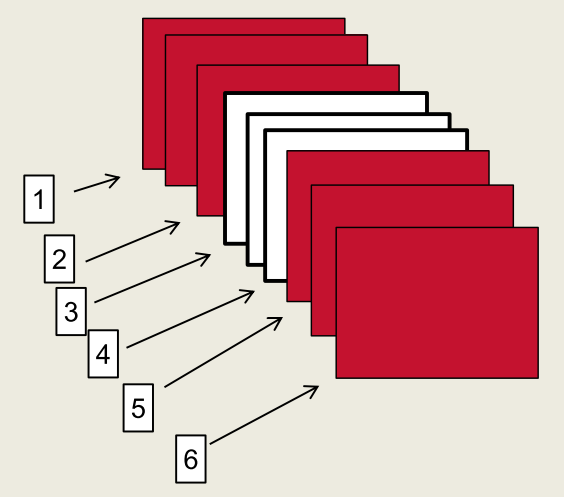
\includegraphics[width=0.4\textwidth]{./figures/eventos.png}
\caption{\small Ejemplo de una secuencia de eventos enumerados. Los colores rojo y blanco indican que el evento tiene poca o mucha relevancia, respectivamente. Eventos del 3 al 4 conforman un episodio interesante para recordar, mientras que el resto pueden servir como pista o consecuencia del episodio. Obtenido de \cite{Kelley2014}.}
\label{img:sleep_eventos}
\end{figure}


%Ejemplo:
%At some location (cue), something big and orange (Tiger) moved from left to right resulting in pain (event)



%Abstraccion de episodios de manera declarativa simbolica... permite mejorar tiempos de busqueda


Además, este diseño permite que el sistema cambie su opinión sobre una evento, mediante aprendizaje reforzado. Si se repiten eventos, pero la consecuencia deja de ser la misma, entonces el sistema se acostumbra.

%\subsubsection{Frameworks relacionados}
%
%... ISAC \cite{Dodd2005}
%... MINERVA, LIDA, Neuronal,M SMRTI \cite{Jockel2008}
%... deficiencias de ISAC, EPIROME, \cite{Stachowicz2012}
%... sobre Tecuci, ISAC, SOAR y Ho \cite{Deutsch2008}
%... definir contenido de QWHAT \cite{Stachowicz2012}
%.. definicion de episodio \cite{Dodd2005}
%... diseno explicado de SONIA en RDF \cite{Vijayakumar2014}

%\todo[inline]{Sobre la memoria procedural}
%\subsection{Memoria Procedural}
%
%... procedural y CRAM \cite{Winkler2014}
%\cite{Winkler2014}

%...... habilidades y PM \cite{Salgado2012}


\subsection{Memoria Emocional}

La importancia de un evento se ve fuertemente influenciada por el estado emocional de una persona. Por lo tanto, la decisión de que almacenar o recordar depende de las emociones\cite{Deutsch2008}.

Su implementación requiere como mínimo de un mapeo entre estímulos percibidos por el robot y las sensaciones emocionales que estos generan. Dood et al. \cite{Dodd2005} propone el uso de la teoría emocional de reacciones de Haikonen, que considera a una emoción como una combinación de estímulos básicos. Las sensaciones elementales son: bienestar, malestar, dolor, placer e interés.

Dood et al. proponen implementar las sensaciones a partir de distintos estímulos medidos en un robot:

\begin{itemize}[topsep=0pt]
\setlength\itemsep{0.2em}
\item Actuador que se aproxima a sus límites de movimiento físico o de fuerza. 
\item Nivel de iluminación percibido.
\item Nivel de ruido acústico percibido.
\item Ausencia o presencia de humanos. Falta de interacción.
\item Cumplimiento de objetivos.
\item Cumplimiento de expectaciones.
\end{itemize}


Sistemas más avanzados, incluso pueden considerar la generación de reacciones emocionales, basándose en las sensaciones derivadas anteriormente. En la figura \ref{img:emotional_haikonen} se muestran las reacciones generadas según el modelo de Haikonen. Además, estas se podrían reflejar en la personalidad del robot, por ejemplo, mediante gestos, vocabulario o nivel de aceptación para realizar una acción. Kasap et al. \cite{Kasap2010} utilizan un sistema llamado \textit{Emotion Engine}, para generar reacciones emocionales y simular cambios de personalidad de un robot, según las sensaciones percibidas.

\begin{figure}[H]
\centering
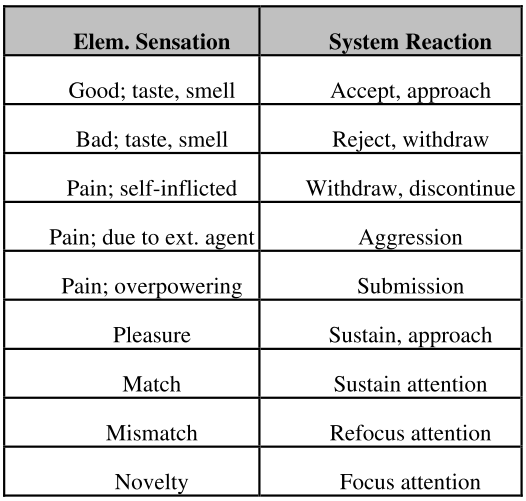
\includegraphics[width=0.4\textwidth]{./figures/haikonen.png}
\caption{\small Sensaciones elementales y sus reacciones correspondientes, según el modelo de Haikonen. Obtenido de \cite{Dodd2005}.}
\label{img:emotional_haikonen}
\end{figure}

Para su uso efectivo dentro de un esquema LTM, se espera que las sensaciones reportadas incluyan un nivel de intensidad. Según el nivel percibido en cada episodio, es posible clasificarlos entre eventos muy o poco relevantes. Los más relevantes tendrán mayor probabilidad de ser recuperados al recordar. Deutsch et al. \cite{Deutsch2008} consideran que el la intensidad de las sensaciones es importante, pues permite evitar costos de búsqueda lineales dentro de todos los episodios almacenados. Por otro lado, Dood et al. proponen curvas de decaimiento para la importancia de los episodios, que permiten simular la pérdida de interés en los eventos.


%... + refs sobre emociones \cite{Deutsch2008}


%\todo[inline]{Resumen de dificultades ... diagrama o tabla.}


\subsection{Otros enfoques}

Se han desarrollado otras derivaciones de la memoria Ep-LTM. Algunos estudios tienen otros objetivos, como el traspaso de memoria entre robots o conflictos éticos con la información. Mientras que otras memorias no se diseñan con un enfoque biológico, basado en la memoria humana.

El sistema propuesto por Ho et al. \cite{Ho2009} busca modelar la memoria de forma suficientemente general, como para permitir el traspaso de los recuerdos de un robot a otro, independientemente de que el hardware sea distinto; El costo de esto, es que se reduce la personalización de cada robot. Ho et al. además aplican la teoría \textit{Roboética}, sugerida por Veruggio y Operto \cite{Veruggio2006}, de donde derivan restricciones de diseño, relativas al manejo de información privada de los usuarios.

En \cite{KimMinJoo2016}, Kim et al. plantean el uso de Deep Learning para modelar la memoria episódica y la planificación de acciones de manera holística. En su implementación, los procesos de codificación, almacenado y recuperación de episodios son manejados como uno solo. Los procesos de decaimiento y relevancia son abstraídos, para ser manejados automáticamente por la red.

Thorsten et al. \cite{Spexard2008} proponen una memoria LTM para el robot BIRON. En su trabajo, se abstraen de la clasificación entre memorias Ep-LTM y S-LTM, pues todos los datos de largo plazo almacenados por el robot son considerados LTM. La memoria almacena sólo datos de alto nivel, obtenidos tras el procesamiento de streams de datos básicos, como cámaras, micrófonos o actuadores. Los datos almacenados corresponden a un historial de percepciones y acciones de alto nivel realizadas, como: detecciones de objetos, interacciones verbales o la descripción de movimientos realizados. A pesar de su simplicidad, esta arquitectura centralizada permite reducir el las dependencias entre si de cada componente y reducir el ancho de banda utilizado para retransmitir la información entre procesos.


\todo[inline]{\cite{Pratama2014}}


% ================================================================
% ================================================================
% ================================================================

\section{Componentes de software}

La implementación de un sistema de memoria robótica asume que muchos sistemas y capacidades de un robot están disponibles. Entonces, se requiere del uso de variados frameworks y librerías que permiten comunicarse con el robot y acceder a los datos de interés que se desea recordar. A continuación se explican los componentes de software relevantes para el trabajo.

\subsection{ROS}

Los sistemas robóticos actuales son cada vez más complejos. Deben lidiar con muchos componentes tanto de hardware como de software y su interacción, de una forma eficaz y que no entorpezca el desarrollo. Muchas tareas de control requieren altas frecuencias de funcionamiento, así como la sincronización y comunicación entre los diversos módulos. Por lo tanto, el cómo se unen los subsistemas en una aplicación robótica es una tarea difícil.

ROS\cite{ROS:2009}, acrónimo para Robot Operating System, es un proyecto que funciona como middleware para aplicaciones robóticas, y permite resolver el problema de la comunicación entre procesos. Es una colección de herramientas, librerías y convenciones que buscan simplificar la tarea de crear comportamientos robóticos complejos y robustos, sin importar la plataforma robótica.

Fue originalmente creado por la organización WillowGarage en el 2008, y mantenido actualmente por la Open Source Robotics Foundation (OSRF). Existe un ecosistema ROS, mantenido por la comunidad, y con cientos de módulos de software con soluciones a problemas específicos, los que pueden interconectarse para construir comportamientos más complejos. Por lo anterior, su uso se ha convertido en una práctica mundial, siendo adoptado incluso en soluciones industriales.

%\todo[inline]{Más información sobre ROS. Lo que sea relevante para la implementación y el diseño.}

%\subsubsection{Nodo}
%
%Mensajes y master
%
%\subsubsection{Tópicos}
%
%\subsubsection{Servicios}
%
%\subsubsection{Servidor de parámetros}
%
%\subsubsection{Launch}

%\subsubsection{Herramientas}

%\subsubsection{Actionlib}


%\subsection{SMACH}

%\todo[inline]{Sobre librería para máquinas de estado (a utilizar en la demostración)}


\subsection{UChile ROS Framework}

UChile ROS Framework (URF) hace referencia al sistema de software desarrollado en el laboratorio de robótica del Departamento de Ingeniería Eléctrica de la Universidad de Chile, para sus robots de servicio. El sistema cuenta con 10 años de desarrollo y está orientado a cumplir los requisitos de la competencia Robocup en su categoría @Home.

URF está construido sobre ROS y en una estructura de 4 capas. La primera capa contiene todas las dependencias del sistema, ya sean de ROS o no; Es la única capa donde que contiene código externo. Sobre ella, se monta una capa ROS de bajo nivel, con herramientas y librerías comunes, sumado a los drivers necesarios para manejar cada robot. La capa intermedia alberga capacidades robóticas avanzadas, relacionadas a percepción robótica, manipulación de objetos, navegación autónoma e interacción Humano-Robot. Finalmente, existe una capa desarrollada en python, con interfaces para el uso de las capacidades de menor nivel, utilizada para la elaboración de maquinas de estado y comportamientos robóticos complejos.

\begin{figure}[H]
\centering
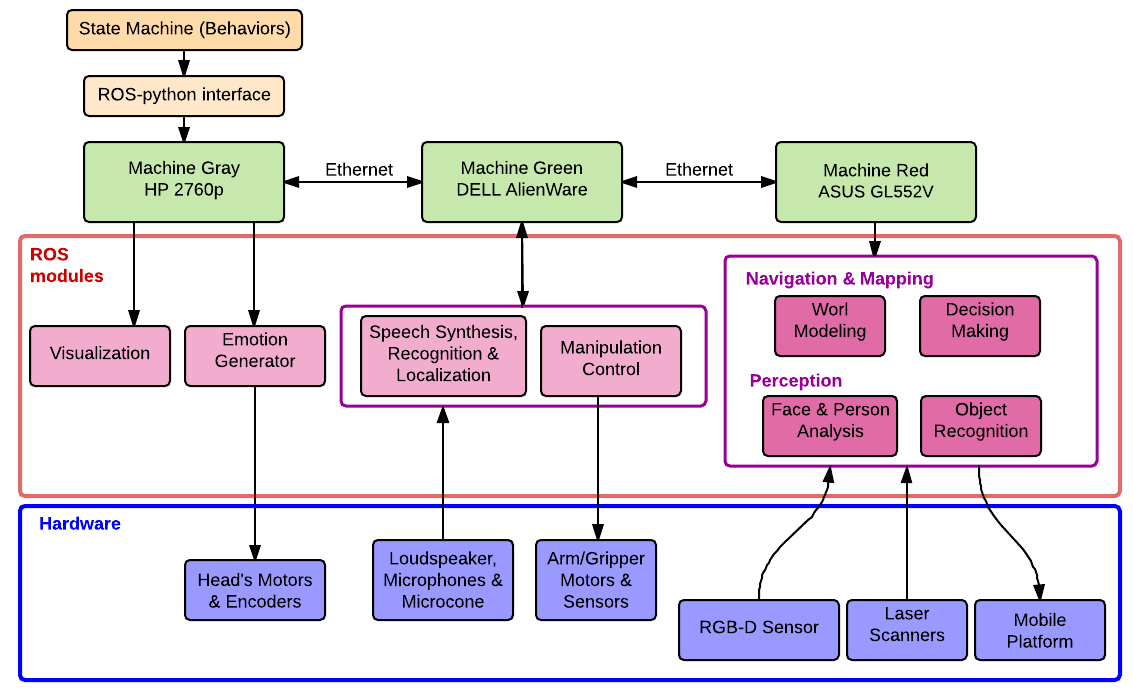
\includegraphics[width=0.8\textwidth]{./figures/URF.png}
\caption{\small Diagrama de UChile ROS Framework utilizado en el robot Bender.}
\label{img:URF}
\end{figure}

Todos los módulos de URF son de código libre, a excepción de los algoritmos relacionados con percepción y la interfaz de alto nivel. El código se almacena públicamente en la organización \textit{uchile-robotics} en GitHub\footnote{Organización \textit{uchile-robotics} y URF en GitHub: \url{https://github.com/uchile-robotics}}.


%\subsubsection{Concepto de robot-skills}
\todo[inline]{Sobre concepto de robot skills y cómo permiten acceder a componentes del robot. Serán utilizadas para la demo.}


\subsubsection{Manejo de información en URF}

Si un robot implementa URF, entonces es posible acceder a la información compartida por sus procesos. Cualquier módulo ROS en el sistema tiene acceso a los datos extraídos desde sensores y luego generados en post-procesamientos, junto al acceso para controlar el hardware.

Existen algunas formas de memoria implementadas en URF, comparables a los conceptos definidos para la memoria humana. También se pueden dividir en de corto y largo plazo:

Como STM, se puede definir como memoria de trabajo a todo el flujo de información presente durante la ejecución del robot. Lo que incluye datos sensados, procesamientos y acciones realizadas. Generalmente tales datos no son almacenados para posteriores ejecuciones.

A manera de LTM, se puede encontrar una memoria procedural, relacionada con todo el conocimiento almacenado que posee el robot para cumplir ciertas tareas. Caen en esta categoría: modelos para percepción robótica, modelos para reconocimiento de voz y patrones, bases de datos de movimientos precalculados para manipular objetos y acciones predefinidas que se utilizan para controlar el robot.

También se pueden encontrar especializaciones de memoria LTM semántica. Ejemplos de esto son: El mapa que se conoce del entorno, junto a los lugares y objetos anotados en él. Diccionarios con información anotada sobre entidades y sus características, cómo personas y objetos. Bases de datos con imágenes anotadas para el reconocimiento de objetos y personas. 

Sin embargo, en URF no existen formas de memoria emocional ni episódica de largo plazo. Luego, toda interacción realizada por los robots está limitada a la información obtenida desde el inicio al término de cada rutina.



\subsection{KnowRob}

KnowRob es un sistema de procesamiento de conocimiento. Combina métodos para representar conocimiento y para razonar a partir de él, junto a técnicas  para adquirir conocimiento y almacenarlo físicamente. Permite integrar información proveniente de distintas fuentes\cite{Tenorth2013, Tenorth2009}.

Está implementado en java, prolog y provee una interfaz ROS. Almacena los datos en archivos OWL (Web Ontology Language) y en una base de datos NoSQL, MongoDB. Por su diseño, permite el manejo e inferencia de memoria semántica y procedural.


\todo[inline]{Más info sobre knowRob... todo el trabajo se basará en este software!.}

\todo[inline]{Sobre OWL... utilizado por KnowRob.}

\todo[inline]{Sobre Prolog... utilizado por KnowRob.}

\todo[inline]{Sobre MongoDB... utilizada por KnowRob.}

% ================================================================
% ================================================================
% ================================================================


\section{Plataformas objetivo}

\subsection{Robot Bender}

Bender es un robot humanoide creado el año 2007 en el laboratorio de robótica del Departamento de Ingeniería Eléctrica de la Universidad de Chile. El equipo UChile Homebreakers es el encargado de su desarrollo y  su objetivo es ser un mayordomo para el hogar, funcionando de manera autónoma para apoyar en tales labores\cite{uchile-robotics}.

\begin{figure}[H]
\centering
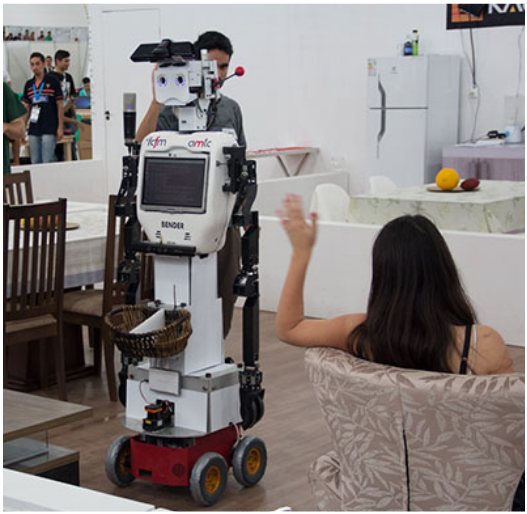
\includegraphics[width=0.5\textwidth]{./figures/bender.png}
\caption{\small Robot Bender en competencia RoboCup 2015.}
\label{img:bender}
\end{figure}


En cuanto a actuadores, el robot cuenta con 2 brazos antropomórficos de 6 grados de libertad cada uno, una base móvil diferencial Pioneer 3-AT, un cuello que permite rotaciones en dos ejes cartesianos; pudiendo imitar gestos de asentimiento y negación, y finalmente, una cabeza que puede mostrar expresiones faciales mediante movimientos de su boca, orejas, cejas y cambios de colores alrededor de los ojos.

El robot cuenta con los siguientes sensores: un laser Hokuyo UTM-30LX, un laser Hokuyo URG-04LX-UG01, un micrófono M-Audio Producer USB y una cámara de profundidad ASUS Xtion Pro.

El software de Bender está basado en el framework URF. Su arquitectura de software utiliza  ROS para el manejo de componentes de bajo y medio nivel. La capa de alto nivel, escrita en python, se abstrae de ROS y permite la creación de comportamientos complejos mediante máquinas de estado. Todos los módulos que interactúan con sensores y actuadores están implementados en ROS.



%\todo[inline]{Robot pepper es eliminado por ahora, para acotar los alcances.}
%\subsection{Pepper}
%
%Pepper es un robot humanoide desarrollado por SoftBank Robotics, orientado a la interacción humano robot y con el objetivo de ser un robot de compañía y soporte emocional.


%\section{Contribución del Trabajo}



